\documentclass[a4paper, 12pt, oneside]{report}

\usepackage{preamble}

\begin{document}

\noindent \textbf{Práctica 6} \hfill \textbf{David López del Pino}

\hfill

En esta práctica se implementa un esquema en diferencias finitas explícito para la ecuación del calor. El esquema es el siguiente:
\[u_i^{n+1} = u_i^n + \frac{k\Delta t}{\Delta x^2}(u_{i+1}-2u_i^n + u_{i-1}^n) + \Delta t F(x_i, t_n),\]
donde $F$ es el término fuente y $k$ es el coeficiente de difusión. Este esquema es estable bajo la condición CFL $\Delta t \leq \frac{\Delta x^2}{2k}$.

Resolveremos la ecuación en el intervalo $[0,10]$ con tiempo máximo $T = 20$ y tomando $\Delta x = 0'5$ y $k = 1$. Con el dato inicial $f(x) = \sin(\frac{\pi x}{10})$, la solución exacta del problema es $u(x,t) = \sen(\frac{\pi x}{10})\exp(-(\frac{\pi}{10})^2t)$. 

Primero consideramos condiciones de Dirichlet homogéneas en los extremos. Tomando $\Delta t = 0'2$, no se verifica la condición CFL porque $\frac{\Delta x^2}{2k} = 0'125$. Al ejecutar la función \texttt{calor\_dirichlet} con estos datos se observa que la solución aproximada explota alrededor de $t = 10$.
\begin{center}
    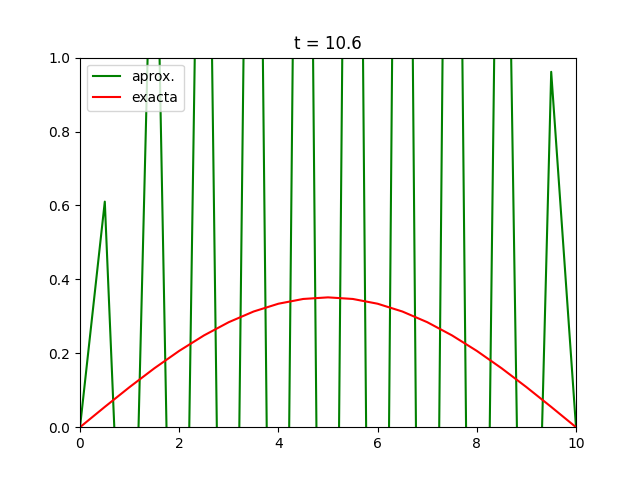
\includegraphics[scale = 0.8]{./images/Figure_1.png}
\end{center}
Tomando $\Delta t = 0'125$, sí se verifica la condición CFL y al ejecutar la función anterior se observa que la gráfica de la solución aproximada coincide con la de la solución exacta.
\begin{center}
    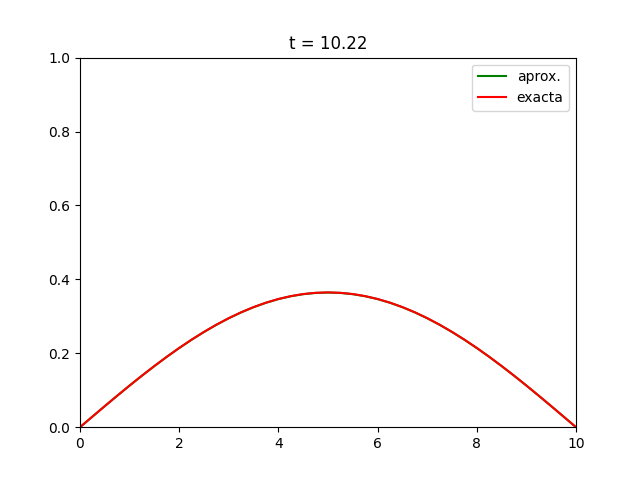
\includegraphics[scale = 0.8]{./images/Figure_2.png}
\end{center}
Ahora comparamos el error cometido con $\Delta x = 0'5$ y $\Delta x = 0'25$. En ambos casos, se toma $\Delta t = \frac{\Delta x^2}{2}$ para que se verifique la condición CFL.
\begin{center}
    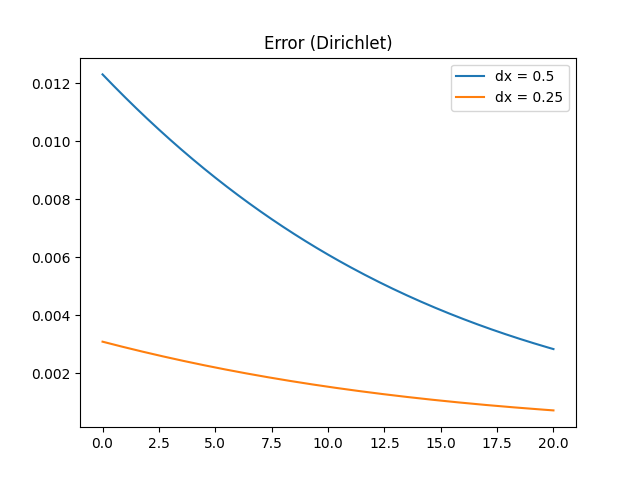
\includegraphics[scale = 0.8]{./images/Figure_3.png}
\end{center}
Vemos que al reducir $\Delta x$ a la mitad, el error cometido es aproximadamente cuatro veces menor. Esto ocurre porque el esquema empleado es de orden $2$ en $x$.

A continuación, construimos un problema con condiciones de Neumann en los extremos que siga teniendo a $u(x,t) = \sen(\frac{\pi x}{10})\exp(-(\frac{\pi}{10})^2t)$ como solución exacta. Para obtener las condiciones de Neumann, derivamos $u$ respecto de $x$ y evaluamos en los extremos: 
\[\begin{aligned}
u_x(0,t) &= \frac{\pi}{10}\exp\bigl(-\bigl(\frac{\pi}{10}\bigr)^2t\bigr),\\
u_x(10,t) &= -\frac{\pi}{10}\exp\Bigl(-\Bigl(\frac{\pi}{10}\Bigr)^2t\Bigr).
\end{aligned}
\]
Ahora ejecutamos la función \texttt{calor\_neumann} con $\Delta x = 0'5$ y $\Delta x = 0'25$, tomando en ambos casos $\Delta t = \frac{\Delta x^2}{2}$ para que se cumpla la condición CFL.
\begin{center}
    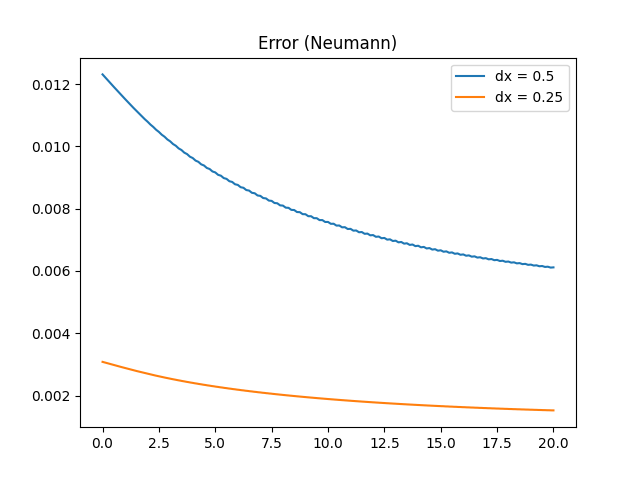
\includegraphics[scale = 0.8]{./images/Figure_4.png}
\end{center}
De nuevo, al reducir $\Delta x$ a la mitad se comete un error aproximadamente cuatro veces menor, y esto se debe a que el esquema es de orden $2$ en $x$.

\end{document}